
\subsubsection{Citation}

A citation network represented as a directed unweighted graph, with nodes representing individual documents and edges indicating a citation from one document to another.

\begin{figure}[H]
    \centering
    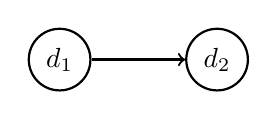
\begin{tikzpicture}[node distance=2cm, thick, main/.style = {draw, circle}]
        \node[main] (1) [] {$d_1$};
        \node[main] (2) [right of=1] {$d_2$};
        \draw[->] (1) -- (2);
    \end{tikzpicture}
    \caption{Citation} \label{fig:citation}
\end{figure}

Figure \ref{fig:citation} depicts a citation diad in which document $d_1$ cites document $d_2$.

\subsubsection{Co-Citation}

A co-citation network represented as an undirected weighted graph, with nodes corresponding to individual documents and edge weights representing the frequency with which two documents are co-cited.

\citep{small1973,small1974,griffith1974,small1977,small1979}

\begin{figure}[H]
    \centering
    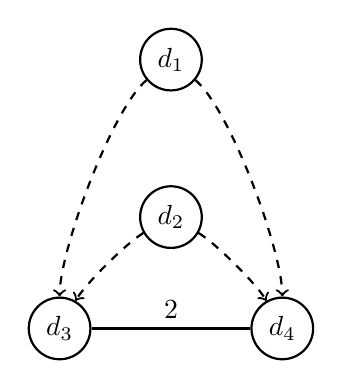
\begin{tikzpicture}[node distance=2cm, thick, main/.style = {draw, circle}]
        \node[main] (1) [] {$d_1$};
        \node[main] (2) [below of=1] {$d_2$};
        \node[main] (3) [below left of=2] {$d_3$};
        \node[main] (4) [below right of=2] {$d_4$};
        \draw[->] (1) to [out=220, in=90, looseness=0.5] (3) [dashed] node {};
        \draw[->] (1) to [out=320, in=90, looseness=0.5] (4) [dashed] node {};
        \draw[->] (2) to [out=210, in=60, looseness=0.5] (3) [dashed] node {};
        \draw[->] (2) to [out=330, in=120, looseness=0.5] (4) [dashed] node {};
        \draw[] (3) -- node[midway, above] {2} (4);
    \end{tikzpicture}
    \caption{Co-Citation} \label{fig:co_citation}
\end{figure}

As shown in Figure \ref{fig:co_citation}, the edge weight of 2 between documents $d_3$ and $d_4$ reflects the fact that they are co-cited by two documents, $d_1$ and $d_2$.

\subsubsection{Co-Occurrence}

A co-occurrence network represented as an undirected weighted graph, with nodes representing individual terms and edge weights indicating the frequency with which two terms co-occur within a document.

\input{figures/co_occurrence}

As shown in Figure \ref{fig:co_occurrence}, the edge weight of 2 between terms $w_3$ and $w_4$ 
reflects the fact that they co-occur in both documents, $d_1$ and $d_2$.
